\section{Server}
Il server ha una struttura multi-thread: ogni nuova connessione viene gestita da un differente \textit{TCPRequestHandler}\footnote{Che eredita da \textit{Runnable}}, il cui ciclo di vita viene incapsulato all'interno di un \textit{ThreadPoolExecutor}\footnote{Si è scelto di utilizzare un ThreadPoolExecutor di tipo \textit{CachedThreadPool}}. 

\begin{lstlisting}[caption="Gestione di una nuova connessione", language=java]
while(true) {
	Socket socket = TCPServer.accept();
	System.out.println("New TCP connection: " + socket.getRemoteSocketAddress().toString());
	TCPConnectionDispatcher.submit(new TCPRequestHandler(onlineUsersDB, usersDB, documentDatabase, cdaManager, socket));
}
\end{lstlisting}

L'oggetto Server, attraverso il metodo \textit{bootstrap}, effettua l'inizializzazione di tutti gli oggetti interni necessari all'esecuzione del ciclo di vita dell'applicazione e tutte le proprietà, considerando le impostazioni scelte dall'utente in fase di avvio del processo\footnote{L'ordine di priorità delle impostazioni è il seguente: riga di comando $\succ$ file di configurazione $\succ$ valori di default}:
\begin{itemize}
	\item Inizializzazione dei valori delle configurazioni;
	\item Controllo della directory di lavoro del server\footnote{Controlla se la directory esiste ed è valida, altrimenti la crea};
	\item Carica le informazioni del database degli utenti\footnote{Astratto dalla classe \textit{UsersDB}};
	\item Carica le informazioni del database dei documenti\footnote{Astratto dalla classe \textit{DocumentsDatabase}};
	\item Configura lo stub RMI per la chiamata \textit{register} remota;
	\item Registra un handler per gestire la chiusura del processo.
\end{itemize}

\paragraph{Persistenza delle informazioni}
Come detto procedentemente, il server inizializza il database dei documenti e quello degli utenti effettuando una ricerca all'interno della cartella di lavoro per trovare i file \textbf{db.dat} e \textbf{docs.dat}. Se questi vengono individuati, Server tenta di effettuare una deserializzazione per ricostruire gli oggetti originali, altrimenti vengono utilizzati degli oggetti vergini non contenenti alcun dato.

La serializzazione degli oggetti, invece, avviene all'interno della routine associata all'hook di terminazione, che viene richiamata in fase di terminazione del processo.

\paragraph{Sessione}
Si è deciso di gestire lo scambio di messaggi tra client e server mantenendo attiva una connessione TCP persistente, ma sfruttando comunque un meccanismo di identificazione univoco della sessione \footnote{Per \textit{sessione} s'intende tutta la sequenza di comandi TURING che intercorrono tra una richiesta di login e la rispettiva richiesta di logout} attraverso l'impiego un token, che viene generato dal Server in seguito alla richiesta di login \footnote{Il token è una stringa a 256-bit formata dallo SHA-256 della concatenazione del timestamp della richiesta e dell'hash della password dell'utente} e distrutto in seguito a quella di logout. La motivazione che sta dietro a questa scelta implementativa è quella di porre alla base del meccanismo di identificazione una struttura quanto più semplice da modificare e da ampliare: così strutturata, è possibile lasciare la possibilità di implementare un meccanismo che permetta di impiantare direttamente il token all'apertura del client e di poter così permettere ad altri di utilizzare il proprio "profilo" senza la necessità di fornire le proprie credenziali in chiaro.

\paragraph{Thread Life-cycle}
Alla richiesta di connessione da parte del client sul socket principale, il server smista il canale sul socket secondario e passa il suo riferimento al \textit{TCPRequestHandler}, il quale si occuperà di effettuare il dispatching dei comandi e richiamerà gli opportuni handler. Alla richiesta di \textbf{login}, il server creerà una nuova istanza del \textit{NotificationServerThread}\footnote{Questo, a differenza di quanto si potrebbe immaginare, in realtà funge da \underline{client} per una "reverse connection" che viene instaurata allo specifico scopo di gestire richieste e risposte relative al pulling di notifiche}, che rimarrà attivo per tutto il tempo della durata della sessione.
\begin{figure}[h]
	\caption{Server - Ciclo di vita dei Thread}
	\centering
	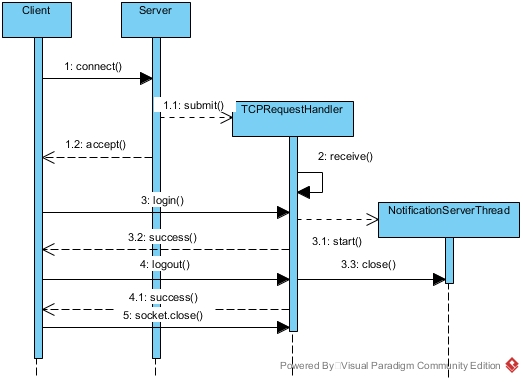
\includegraphics[scale=0.5]{assets/server/thread_activation_sequence_diagram}
\end{figure}